\documentclass{scrartcl}
        \usepackage{xcolor, tikz}
        \usepackage{pgfplots}
        \pgfplotsset{compat=newest}
        \pagestyle{empty}
        \definecolor{pdg2112}{RGB}{228,26,28}
\definecolor{pdg2212}{RGB}{55,126,184}
\definecolor{pdg1000010020}{RGB}{153,153,153}
\definecolor{pdg1000020040}{RGB}{166,86,40}
\definecolor{pdg11}{RGB}{152,78,163}
\definecolor{pdg12}{RGB}{255,127,0}
\definecolor{pdg1000010030}{RGB}{153,153,153}
\definecolor{pdg1000060120}{RGB}{153,153,153}
\definecolor{pdg1000040090}{RGB}{153,153,153}
\begin{document}
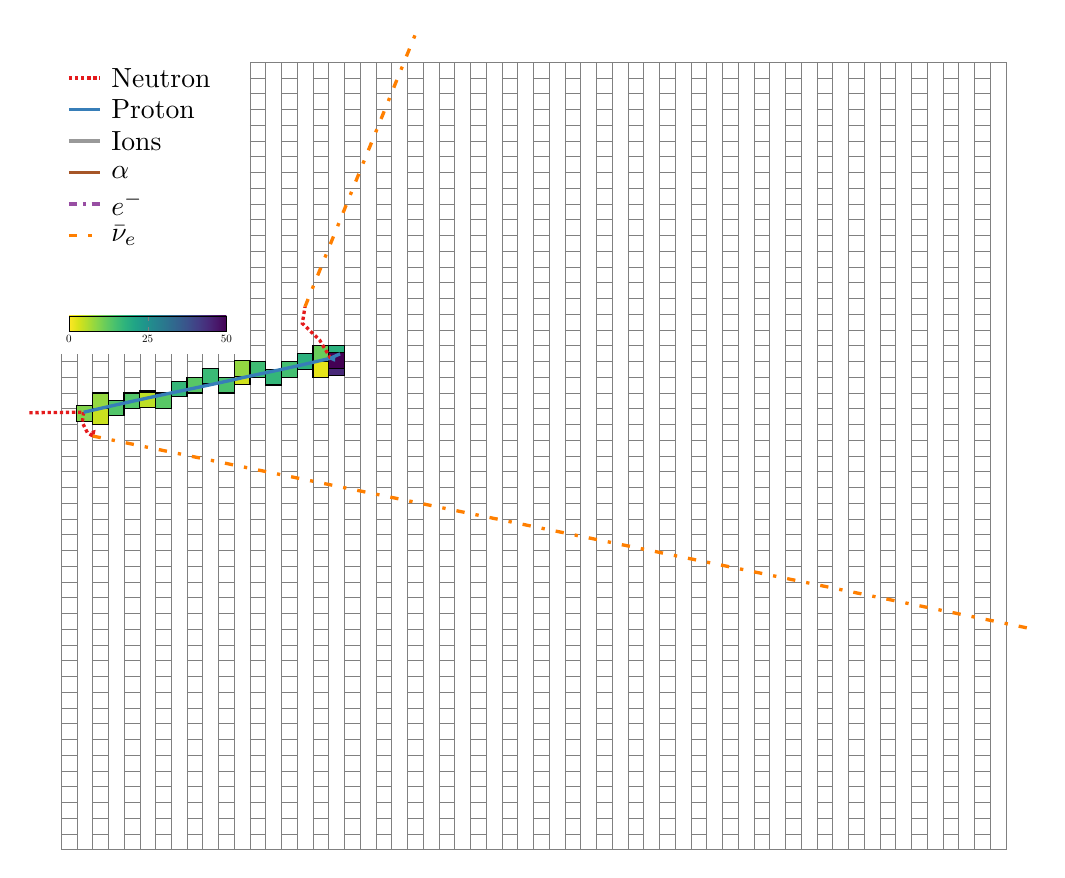
\begin{tikzpicture}[scale=0.4] %\columnwidth/252.0pt]
\draw[step=0.5,very thin,gray] (-0.001000,-12.499) grid (0.500000,3.25);
\draw[step=0.5,very thin,gray] (0.999000,-12.499) grid (1.500000,3.25);
\draw[step=0.5,very thin,gray] (1.999000,-12.499) grid (2.500000,3.25);
\draw[step=0.5,very thin,gray] (2.999000,-12.499) grid (3.500000,3.25);
\draw[step=0.5,very thin,gray] (3.999000,-12.499) grid (4.500000,3.25);
\draw[step=0.5,very thin,gray] (4.999000,-12.499) grid (5.500000,3.25);
\draw[step=0.5,very thin,gray] (5.999000,-12.499) grid (6.500000,12.499);
\draw[step=0.5,very thin,gray] (6.999000,-12.499) grid (7.500000,12.499);
\draw[step=0.5,very thin,gray] (7.999000,-12.499) grid (8.500000,12.499);
\draw[step=0.5,very thin,gray] (8.999000,-12.499) grid (9.500000,12.499);
\draw[step=0.5,very thin,gray] (9.999000,-12.499) grid (10.500000,12.499);
\draw[step=0.5,very thin,gray] (10.999000,-12.499) grid (11.500000,12.499);
\draw[step=0.5,very thin,gray] (11.999000,-12.499) grid (12.500000,12.499);
\draw[step=0.5,very thin,gray] (12.999000,-12.499) grid (13.500000,12.499);
\draw[step=0.5,very thin,gray] (13.999000,-12.499) grid (14.500000,12.499);
\draw[step=0.5,very thin,gray] (14.999000,-12.499) grid (15.500000,12.499);
\draw[step=0.5,very thin,gray] (15.999000,-12.499) grid (16.500000,12.499);
\draw[step=0.5,very thin,gray] (16.999000,-12.499) grid (17.500000,12.499);
\draw[step=0.5,very thin,gray] (17.999000,-12.499) grid (18.500000,12.499);
\draw[step=0.5,very thin,gray] (18.999000,-12.499) grid (19.500000,12.499);
\draw[step=0.5,very thin,gray] (19.999000,-12.499) grid (20.500000,12.499);
\draw[step=0.5,very thin,gray] (20.999000,-12.499) grid (21.500000,12.499);
\draw[step=0.5,very thin,gray] (21.999000,-12.499) grid (22.500000,12.499);
\draw[step=0.5,very thin,gray] (22.999000,-12.499) grid (23.500000,12.499);
\draw[step=0.5,very thin,gray] (23.999000,-12.499) grid (24.500000,12.499);
\draw[step=0.5,very thin,gray] (24.999000,-12.499) grid (25.500000,12.499);
\draw[step=0.5,very thin,gray] (25.999000,-12.499) grid (26.500000,12.499);
\draw[step=0.5,very thin,gray] (26.999000,-12.499) grid (27.500000,12.499);
\draw[step=0.5,very thin,gray] (27.999000,-12.499) grid (28.500000,12.499);
\draw[step=0.5,very thin,gray] (28.999000,-12.499) grid (29.500000,12.499);
\draw[very thin,gray] (0,-12.5) -- (30,-12.5) -- (30,12.5) -- (6,12.5);
\definecolor{tempcolor}{rgb}{0.506271,0.828786,0.300362}\draw[fill=tempcolor,fill opacity=1] (0.500000,1.101024) rectangle (1.000000,1.601024);
\definecolor{tempcolor}{rgb}{0.793760,0.880678,0.120005}\draw[fill=tempcolor,fill opacity=1] (1.000000,1.000000) rectangle (1.500000,1.500000);
\definecolor{tempcolor}{rgb}{0.585678,0.846661,0.249897}\draw[fill=tempcolor,fill opacity=1] (1.000000,1.500000) rectangle (1.500000,2.000000);
\definecolor{tempcolor}{rgb}{0.319809,0.770914,0.411152}\draw[fill=tempcolor,fill opacity=1] (1.500000,1.273730) rectangle (2.000000,1.773730);
\definecolor{tempcolor}{rgb}{0.319809,0.770914,0.411152}\draw[fill=tempcolor,fill opacity=1] (2.000000,1.500000) rectangle (2.500000,2.000000);
\definecolor{tempcolor}{rgb}{0.762373,0.876424,0.137064}\draw[fill=tempcolor,fill opacity=1] (2.500000,1.575120) rectangle (3.000000,2.075120);
\definecolor{tempcolor}{rgb}{0.741388,0.873449,0.149561}\draw[fill=tempcolor,fill opacity=1] (2.500000,1.532795) rectangle (3.000000,2.032795);
\definecolor{tempcolor}{rgb}{0.344074,0.780029,0.397381}\draw[fill=tempcolor,fill opacity=1] (3.000000,1.500000) rectangle (3.500000,2.000000);
\definecolor{tempcolor}{rgb}{0.208030,0.718701,0.472873}\draw[fill=tempcolor,fill opacity=1] (3.500000,1.876917) rectangle (4.000000,2.376917);
\definecolor{tempcolor}{rgb}{0.344074,0.780029,0.397381}\draw[fill=tempcolor,fill opacity=1] (4.000000,2.000000) rectangle (4.500000,2.500000);
\definecolor{tempcolor}{rgb}{0.226397,0.728888,0.462789}\draw[fill=tempcolor,fill opacity=1] (4.500000,2.284508) rectangle (5.000000,2.784508);
\definecolor{tempcolor}{rgb}{0.288921,0.758394,0.428426}\draw[fill=tempcolor,fill opacity=1] (5.000000,2.000000) rectangle (5.500000,2.500000);
\definecolor{tempcolor}{rgb}{0.814576,0.883393,0.110347}\draw[fill=tempcolor,fill opacity=1] (5.500000,2.262994) rectangle (6.000000,2.762994);
\definecolor{tempcolor}{rgb}{0.575563,0.844566,0.256415}\draw[fill=tempcolor,fill opacity=1] (5.500000,2.530487) rectangle (6.000000,3.030487);
\definecolor{tempcolor}{rgb}{0.246070,0.738910,0.452024}\draw[fill=tempcolor,fill opacity=1] (6.000000,2.500000) rectangle (6.500000,3.000000);
\definecolor{tempcolor}{rgb}{0.202219,0.715272,0.476084}\draw[fill=tempcolor,fill opacity=1] (6.500000,2.255038) rectangle (7.000000,2.755038);
\definecolor{tempcolor}{rgb}{0.266941,0.748751,0.440573}\draw[fill=tempcolor,fill opacity=1] (7.000000,2.500000) rectangle (7.500000,3.000000);
\definecolor{tempcolor}{rgb}{0.170948,0.694384,0.493803}\draw[fill=tempcolor,fill opacity=1] (7.500000,2.754088) rectangle (8.000000,3.254088);
\definecolor{tempcolor}{rgb}{0.896320,0.893616,0.096335}\draw[fill=tempcolor,fill opacity=1] (8.000000,2.500000) rectangle (8.500000,3.000000);
\definecolor{tempcolor}{rgb}{0.412913,0.803041,0.357269}\draw[fill=tempcolor,fill opacity=1] (8.000000,3.000000) rectangle (8.500000,3.500000);
\definecolor{tempcolor}{rgb}{0.170948,0.694384,0.493803}\draw[fill=tempcolor,fill opacity=1] (8.500000,3.003902) rectangle (9.000000,3.503902);
\definecolor{tempcolor}{rgb}{0.281412,0.155834,0.469201}\draw[fill=tempcolor,fill opacity=1] (8.500000,2.567302) rectangle (9.000000,3.067302);
\definecolor{tempcolor}{rgb}{0.267004,0.004874,0.329415}\draw[fill=tempcolor,fill opacity=1] (8.500000,2.777215) rectangle (9.000000,3.277215);
\draw[color=pdg2112, very thick, densely dotted] (-1.00669324096109, 1.3734420858139826) -- (-0.006738162041369833, 1.3826598179335394) -- (0.48999999999998634, 1.3872388229386492) -- (0.7173891443857883, 1.3893349293178554);
\draw[color=pdg1000040090, very thick, solid] (0.7173891443857883, 1.3893349293178554);
\draw[color=pdg2112, very thick, densely dotted] (0.7173891443857883, 1.3893349293178554) -- (0.6734613311798284, 1.0644324335910056) -- (0.8415890175877394, 0.7301967529220657) -- (0.9900000000000091, 0.6472200924246885) -- (0.9920000000000073, 0.6472222708494053) -- (0.9899999999999863, 0.6501789919485493) -- (0.984608644838113, 0.6581493587285779) -- (0.9900000000000319, 0.6795091159334969) -- (0.9970000000000028, 0.698426789226152) -- (1.0029999999999972, 0.7146419377627786) -- (1.0080000000000156, 0.7281545615433187) -- (1.0183097534390981, 0.7560169254417064) -- (1.0290791223689666, 0.7585367123761688) -- (1.0100000000000136, 0.6665783660197487) -- (1.0079999999999927, 0.6569386829589476) -- (1.0032703146674067, 0.634142349167511);
\draw[color=pdg11, very thick, dashdotted] (1.0032703146674067, 0.634142349167511);
\draw[color=pdg12, very thick, loosely dashdotted] (1.0032703146674067, 0.634142349167511) -- (1.4899999999999864, 0.5341920082041688) -- (1.9168468049258536, 0.4465386659546625) -- (1.9391206220396726, 0.4419647193017897) -- (1.9582124652800985, 0.43804419359932706) -- (1.9741223346471088, 0.434777088847275) -- (1.9899999999999864, 0.4315165972159908) -- (2.4899999999999864, 0.3288411862278151) -- (2.9899999999999864, 0.2261657752396394) -- (3.4899999999999864, 0.12349036425146369) -- (3.5301075587407467, 0.11525424409658187) -- (3.5491994019811726, 0.11133371839411925) -- (3.565109271348183, 0.10806661364206724) -- (3.990000000000009, 0.02081495326328119) -- (4.042665741287033, 0.009999999999999992) -- (4.052405171500891, 0.007999999999999997) -- (4.076753747035582, 0.0030000000000000217) -- (4.105972037677202, -0.003000000000000021) -- (4.13032061321187, -0.007999999999999997) -- (4.140060043425729, -0.00999999999999999) -- (4.490000000000009, -0.08186045772489588) -- (4.989999999999986, -0.1845358687130669) -- (5.489999999999986, -0.28721127970124266) -- (5.989999999999986, -0.3898866906894184) -- (6.477523294755111, -0.48999999999999994) -- (6.487262724968969, -0.4920000000000001) -- (6.4970000000000026, -0.49399955743143104) -- (6.689807615029099, -0.5335927596609604) -- (6.712081432142918, -0.5381667063138333) -- (6.731173275383344, -0.5420872320162958) -- (6.747083144750354, -0.545354336768348) -- (6.989999999999986, -0.5952375126657721) -- (7.489999999999986, -0.6979129236539477) -- (7.989999999999986, -0.8005883346421234) -- (8.489999999999986, -0.9032637456302991) -- (8.989999999999986, -1.005939156618475) -- (9.489999999999986, -1.1086145676066508) -- (9.871781488431315, -1.1870137100713782) -- (9.894055305545134, -1.1915876567242507) -- (9.913147148785537, -1.1955081824267135) -- (9.929057018152548, -1.1987752871787656) -- (9.989999999999986, -1.2112899785948277) -- (10.489999999999986, -1.3139653895830035) -- (10.989999999999986, -1.416640800571179) -- (11.347238401691266, -1.49) -- (11.356977831905146, -1.492) -- (11.381326407439815, -1.4969999999999999) -- (11.410544698081434, -1.5030000000000001) -- (11.434893273616126, -1.5079999999999998) -- (11.444632703829985, -1.5100000000000002) -- (11.489999999999986, -1.5193162115593564) -- (11.520043954853644, -1.525485762383973) -- (11.989999999999986, -1.6219916225475326) -- (12.489999999999986, -1.7246670335357084) -- (12.989999999999986, -1.8273424445238842) -- (13.489999999999986, -1.9300178555120595) -- (13.989999999999963, -2.0326932665002353) -- (14.489999999999963, -2.135368677488407) -- (14.644742298534675, -2.167145135687003) -- (14.667016115648494, -2.1717190823398758) -- (14.686107958888897, -2.1756396080423386) -- (14.70201782825593, -2.178906712794391) -- (14.990000000000009, -2.238044088476574) -- (15.489999999999963, -2.3407194994647496) -- (15.989999999999963, -2.443394910452921) -- (16.216953508627533, -2.4899999999999998) -- (16.226692938841417, -2.492) -- (16.251041514376084, -2.497) -- (16.280259805017703, -2.503) -- (16.304608380552395, -2.508) -- (16.314347810766275, -2.5100000000000002) -- (16.49000000000001, -2.5460703214410905) -- (16.989999999999963, -2.6487457324292665) -- (17.489999999999963, -2.751421143417437) -- (17.826716171936937, -2.8205660860974158) -- (17.848989989050757, -2.825140032750289) -- (17.868081832291182, -2.8290605584527513) -- (17.883991701658214, -2.832327663204803) -- (17.99000000000001, -2.854096554405606) -- (18.489999999999963, -2.9567719653937816) -- (18.989999999999963, -3.0594473763819527) -- (19.489999999999963, -3.162122787370124) -- (19.989999999999963, -3.2647981983582945) -- (20.489999999999963, -3.367473609346466) -- (20.989999999999963, -3.470149020334637) -- (21.086668615563916, -3.4899999999999998) -- (21.0964080457778, -3.4919999999999995) -- (21.120756621312466, -3.497) -- (21.149974911954086, -3.5029999999999992) -- (21.174323487488778, -3.5080000000000005) -- (21.184062917702658, -3.5099999999999993) -- (21.49000000000001, -3.5728244313228052) -- (21.989999999999963, -3.6754998423109813) -- (22.489999999999963, -3.7781752532991524) -- (22.59967698204041, -3.8006975117130337) -- (22.621950799154227, -3.8052714583659073) -- (22.641042642394655, -3.80919198406837) -- (22.656952511761666, -3.8124590888204226) -- (22.989999999999963, -3.8808506642873235) -- (23.489999999999963, -3.9835260752754946) -- (23.989999999999963, -4.086201486263666) -- (24.489999999999963, -4.188876897251836) -- (24.989999999999963, -4.291552308240008) -- (25.489999999999963, -4.394227719228178) -- (25.781650855442717, -4.454118462123447) -- (25.803924672556537, -4.4586924087763204) -- (25.82301651579696, -4.462612934478783) -- (25.838926385163994, -4.465880039230836) -- (25.99000000000001, -4.496903130216351) -- (26.019690018890447, -4.503) -- (26.044038594425114, -4.507999999999999) -- (26.053778024638994, -4.51) -- (26.49000000000001, -4.599578541204531) -- (26.989999999999963, -4.702253952192706) -- (27.489999999999963, -4.804929363180877) -- (27.989999999999963, -4.907604774169048) -- (28.391241275968422, -4.99) -- (28.400980706182327, -4.991999999999999) -- (28.425329281716994, -4.997) -- (28.454547572358614, -5.003) -- (28.478896147893284, -5.007999999999999) -- (28.488635578107186, -5.01) -- (28.963624728845026, -5.107539412533861) -- (28.985898545958843, -5.112113359186734) -- (29.002999999999997, -5.115625156831075) -- (29.489999999999963, -5.215631007133555) -- (29.989999999999963, -5.318306418121727) -- (30.933202045549773, -5.511993733465154);
\draw[color=pdg2212, very thick, solid] (1.0032703146674067, 0.634142349167511);
\draw[color=pdg2212, very thick, solid] (0.9829847097347738, 0.660550120320416);
\draw[color=pdg2212, very thick, solid] (0.9932187841252471, 0.6454204684801993);
\draw[color=pdg1000060120, very thick, solid] (0.8415890175877394, 0.7301967529220657);
\draw[color=pdg2212, very thick, solid] (0.6734613311798284, 1.0644324335910056);
\draw[color=pdg1000010020, very thick, solid] (0.7173891443857883, 1.3893349293178554);
\draw[color=pdg2212, very thick, solid] (0.7173891443857883, 1.3893349293178554) -- (0.9900000000000091, 1.4506833398555448) -- (1.1632197626584229, 1.49) -- (1.1942697495283028, 1.4969999999999999) -- (1.2207140051000578, 1.5030000000000001) -- (1.242750884743191, 1.5080000000000002) -- (1.490000000000009, 1.5640672706141527) -- (1.9899999999999864, 1.6761719335988854) -- (2.490000000000009, 1.7850069047147894) -- (2.695596926159328, 1.8301894227219475) -- (2.7080254228643073, 1.8328874639495463) -- (2.739465324548064, 1.839654047746242) -- (2.7773076210045473, 1.8478657865876276) -- (2.8088428680516473, 1.8547089022887822) -- (2.821437325219904, 1.8574534350674834) -- (2.9899999999999864, 1.893751923667864) -- (3.443663413637182, 1.9899999999999998) -- (3.477326501465586, 1.9969999999999999) -- (3.5029999999999974, 2.002333396269141) -- (3.811629359093513, 2.0664281625328957) -- (3.9077899655570945, 2.086405006619877) -- (3.9899999999999864, 2.1036254191317756) -- (4.489999999999986, 2.208322086432804) -- (4.693120399753434, 2.2517302491791824) -- (4.990000000000009, 2.3152916294630743) -- (5.490000000000009, 2.4243908631546636) -- (5.766954861296199, 2.4869090302137424) -- (5.779021639303596, 2.489644999074304) -- (5.809412387812131, 2.4965059838742385) -- (5.847674993342617, 2.504612255303326) -- (5.879560497951343, 2.5113674814942324) -- (5.892268477789298, 2.51406586587853) -- (5.990000000000009, 2.534828298116479) -- (6.490000000000009, 2.641114159847306) -- (6.989999999999986, 2.7460965867232163) -- (7.490000000000009, 2.85632823190296) -- (7.990000000000009, 2.971310096566704) -- (8.068621710743718, 2.99) -- (8.09858096587161, 2.9969999999999994) -- (8.124482577279924, 3.003) -- (8.146067253453543, 3.008) -- (8.490000000000009, 3.0882497762164265) -- (8.557853148437289, 3.1039694009427867);
\draw[color=pdg1000010030, very thick, solid] (8.557853148437289, 3.1039694009427867) -- (8.568697139626602, 3.110164620866615) -- (8.577419838161063, 3.1149907832892922);
\draw[color=pdg2112, very thick, densely dotted] (8.557853148437289, 3.1039694009427867) -- (8.510000000000014, 3.1828616996467742) -- (8.497000000000003, 3.2042939338182976) -- (8.323701274788254, 3.4899999999999998) -- (8.20753516759505, 3.6815153240120444) -- (8.010000000000014, 3.8740120610932225) -- (7.714877289802007, 4.161607224239712) -- (7.661440943036905, 4.2069028368061385) -- (7.745921488240174, 4.738391032736295);
\draw[color=pdg11, very thick, dashdotted] (7.745921488240174, 4.738391032736295);
\draw[color=pdg12, very thick, loosely dashdotted] (7.745921488240174, 4.738391032736295) -- (7.885729069571949, 5.08353561003303) -- (7.891056879291955, 5.096688434910056) -- (7.895623573337707, 5.107962284804651) -- (7.899429151709137, 5.117357159716812) -- (7.990000000000009, 5.340950450230701) -- (7.9970000000000026, 5.358231430404011) -- (8.002999999999997, 5.3730436991240165) -- (8.007999999999992, 5.3853872563907) -- (8.05037544386487, 5.49) -- (8.252910251780396, 5.99) -- (8.455445059695922, 6.49) -- (8.489999999999986, 6.575306176897975) -- (8.497000000000003, 6.592587157071343) -- (8.502999999999997, 6.607399425791348) -- (8.507999999999992, 6.619742983058032) -- (8.646844743861948, 6.962510592465341) -- (8.652172553581977, 6.975663417342366) -- (8.656739247627707, 6.986937267236961) -- (8.660544825999159, 6.996332142149122) -- (8.989999999999986, 7.809661903565323) -- (8.997000000000003, 7.82694288373869) -- (9.002999999999997, 7.8417551524586955) -- (9.007999999999992, 7.854098709725379) -- (9.063049483442501, 7.99) -- (9.265584291358028, 8.49) -- (9.468119099273576, 8.99) -- (9.490000000000009, 9.044017630232604) -- (9.497000000000003, 9.061298610405913) -- (9.502999999999997, 9.076110879125919) -- (9.507999999999992, 9.088454436392603) -- (9.788518255297026, 9.780973066113802) -- (9.793846065017055, 9.794125890990827) -- (9.798412759062785, 9.805399740885422) -- (9.802218337434237, 9.814794615797583) -- (9.989999999999986, 10.278373356899888) -- (9.997000000000003, 10.295654337073255) -- (10.002999999999997, 10.310466605793259) -- (10.007999999999992, 10.322810163059943) -- (10.075723523020178, 10.49) -- (10.278258330935728, 10.99) -- (10.480793138851277, 11.49) -- (10.497000000000003, 11.530010063740486) -- (10.502999999999997, 11.54482233246049) -- (10.507999999999992, 11.557165889727173) -- (10.54963392958707, 11.659948048546108) -- (10.5549617393071, 11.673100873423135) -- (10.55952843335283, 11.684374723317728) -- (10.563334011724283, 11.69376959822989) -- (10.930191766732083, 12.59943553976226) -- (10.935519576452112, 12.612588364639288) -- (10.94008627049784, 12.623862214533881) -- (10.943891848869294, 12.633257089446044) -- (10.95769046369644, 12.667321887910012) -- (10.976896198055238, 12.714735304291299) -- (11.3135990870064, 13.545957582615832);
\draw[color=pdg2212, very thick, solid] (7.745921488240174, 4.738391032736295);
\draw[color=pdg2212, very thick, solid] (7.745921488240174, 4.738391032736295);
\draw[color=pdg2212, very thick, solid] (7.714877289802007, 4.161607224239712);
\draw[color=pdg2212, very thick, solid] (8.557853148437289, 3.1039694009427867);
\draw[color=pdg1000020040, very thick, solid] (8.557853148437289, 3.1039694009427867);
\draw[color=pdg2212, very thick, solid] (8.557853148437289, 3.1039694009427867) -- (8.572799522980722, 3.0990398146561544) -- (8.604623413846161, 3.087671222525343) -- (8.626336492841528, 3.0790780264774966) -- (8.642984493931612, 3.0705625729625456) -- (8.655986287729593, 3.0640308665540075) -- (8.667301230402927, 3.0587754963888685) -- (8.67686729515026, 3.0547183264916304) -- (8.683377013020413, 3.052738349530628) -- (8.686950541087299, 3.0515941059898877) -- (8.693828237680282, 3.049578053378613) -- (8.696422264844022, 3.0491875588919943) -- (8.698557319961855, 3.0492011869962763);
\draw[color=pdg1000010020, very thick, solid] (8.557853148437289, 3.1039694009427867);
\draw[color=pdg2212, very thick, solid] (8.557853148437289, 3.1039694009427867) -- (8.625506551066337, 3.136366684727576) -- (8.679096776290043, 3.1611909480318405) -- (8.72097552580783, 3.1810343718521965) -- (8.754678440838735, 3.1963025082171503) -- (8.781641304622644, 3.2078764152018087) -- (8.803653708578532, 3.216735048965382) -- (8.820947843256045, 3.2240515017964753) -- (8.834184369697596, 3.2300454035790254) -- (8.844472411009473, 3.2346929757071288) -- (8.852669874211665, 3.2381104339791067) -- (8.859476990893677, 3.24048700952376);
\draw[color=pdg11, very thick, dashdotted] (4.693120399753434, 2.2517302491791824);
\draw[color=pdg11, very thick, dashdotted] (3.9077899655570945, 2.086405006619877);
\draw[color=pdg11, very thick, dashdotted] (3.811629359093513, 2.0664281625328957);
\draw[color=pdg2112, very thick, densely dotted] (0.25,12) -- (1.25,12) node [right,black] {Neutron};
\draw[color=pdg2212, very thick, solid] (0.25,11) -- (1.25,11) node [right,black] {Proton};
\draw[color=pdg1000010020, very thick, solid] (0.25,10) -- (1.25,10) node [right,black] {Ions};
\draw[color=pdg1000020040, very thick, solid] (0.25,9) -- (1.25,9) node [right,black] {$\alpha$};
\draw[color=pdg11, very thick, dashdotted] (0.25,8) -- (1.25,8) node [right,black] {$e^-$};
\draw[color=pdg12, very thick, loosely dashdotted] (0.25,7) -- (1.25,7) node [right,black] {$\bar{\nu}_e$};

        \begin{axis}[%
            at={(0.25cm,4.75cm)},
            hide axis,
            scale only axis,
            height=0pt,
            width=0pt,
            colormap={reverse viridis}{
                indices of colormap={
                \pgfplotscolormaplastindexof{viridis},...,0 of viridis}
            },
            colorbar horizontal,
            point meta min=0,
            point meta max=50,
            colorbar style={
                width=5cm,
                xtick={50, 25, 0},
            }]
        \end{axis}
        
        \end{tikzpicture}
        \end{document}
        